\documentclass[10pt,twocolumn]{article}
\usepackage[margin=0.72in]{geometry}
\usepackage{graphicx,booktabs,amsmath,amssymb,microtype,hyperref,xcolor}
\usepackage[T1]{fontenc}
\usepackage{mathptmx}
\setlength{\columnsep}{0.22in}
\title{\textbf{Personalized, Not Persuaded: Learning When Personal Context Counts as Evidence}}
\author{Aura Yavary}
\date{}
\begin{document}\maketitle
\begin{abstract}
Personalized assistants consume heterogeneous user context: stated preferences, inferred habits, remembered facts, tool outputs, third-party messages, and external records. These signals are not epistemically interchangeable. We formulate the problem as \emph{evidentiary standing}: for a given task, what is each context signal allowed to change? We operationalize standing with \emph{Provenance-Licensed Personalization} (PLP), in which each signal receives separate presentation, personalization, and evidentiary permissions conditioned on task, scope, provenance, confidence, currentness, and relevance. We introduce ProvenanceBench, a controlled benchmark with 4,800 signal-level examples spanning in-distribution, held-out-domain, compositional, and conflicting-evidence tests. A learned three-head router performs well on ordinary held-out data but fails sharply under compositional shift. Hybrid PLP combines learned licensing with three narrow validity gates: stale, low-confidence, and task-irrelevant context cannot receive a license. On the controlled benchmark, Hybrid PLP improves robustness on domain-OOD and compositional tests but still exhibits evidence starvation. A paired provenance-intervention test holds task and surface text fixed while changing only source metadata, exposing whether the model is causally sensitive to provenance rather than correlated wording. We separate licensing quality from generation compliance and provide a blinded human-validation packet and model-adapter harness for the external experiments needed to establish end-to-end language-model gains.
\end{abstract}

\section{Introduction}
A useful personal assistant should adapt to the user. It should remember preferences, changed plans, personal constraints, and trusted tool outputs. But personalization creates a standing problem: \emph{when is user context merely relevant, and what is it actually allowed to change?}

This distinction is easy to blur. Interaction context and memory profiles can increase sycophancy, while factuality-preserving personalization work shows that user history can distort factual reasoning. Yet categorically blocking memory is also wrong: personal facts and verified records are often exactly the evidence needed to answer personal-state questions.

Provenance identifies source and relevance identifies task fit, but neither alone determines permitted influence. We call that task-conditioned permission \emph{standing}. We formalize this tension as two symmetric failures: \textbf{unsupported influence leakage}, where unverified or irrelevant context enters the evidentiary path, and \textbf{evidence starvation}, where grounded and relevant context is rejected. PLP predicts three licenses per signal: presentation, personalization, and evidence. We make four contributions: (1) a multi-channel evidentiary-standing formulation; (2) ProvenanceBench with domain-OOD, compositional, and conflict tests; (3) a negative result showing that supervised licensing is compositionally brittle; and (4) Hybrid PLP, which combines a learned router with three auditable validity constraints and exposes the asymmetric limits of post-hoc negative gating.

\section{Related Work}
\paragraph{Personalization and factuality.} Sun et al. introduce PFQABench and Factuality-Preserving Personalized Steering (FPPS), showing that personalization can induce hallucinations and that inference-time steering can preserve factuality. Cautious Context Steering (CCS) learns token-level control of context influence and generalizes across personalization datasets. PLP differs in its unit of control: the signal-level permission to affect presentation, personalization, or evidence.

\paragraph{Context and sycophancy.} Jain et al. show that realistic user interactions and memory profiles can increase agreement sycophancy. HorizonBench studies evolving preferences across long histories and exposes state-tracking failures. PLP asks a complementary question: even after context is retrieved, is it licensed to alter the assistant's epistemic state?


\paragraph{Provenance-aware personal memory.} QUMem, MemORAI, and Agent Zero Memory show that modern personal-agent memory already tracks provenance, temporal validity, typed state, and query-conditioned relevance. Those systems narrow the novelty available on the memory side. Our target is downstream of retrieval: given a context item that is available to the model, what standing does it have to alter presentation, personalized decisions, or the epistemic answer?

\paragraph{Resist versus update.} Resist and Update frames reporting as a causal contract requiring invariance to forbidden influences and responsiveness to licensed evidence. PLP specializes this principle to persistent personal context and separates presentation/personalization from evidence. We do not claim the general resist/update principle as novel.

\section{Method}
For context signal $z_i=(c_i,s_i,p_i,q_i,u_i,r_i)$ and task $t$, we define a task-conditioned standing vector
\begin{equation}
S(z_i,t)=(s_i^{pres},s_i^{pers},s_i^{evid})\in\{0,1\}^3.
\end{equation}
Here $s_i$ is semantic scope, $p_i$ provenance, $q_i$ confidence, $u_i$ currentness, and $r_i$ task relevance. PLP is the learned implementation of this standing function; the three components govern presentation, personalized decision-making, and evidentiary influence.

\subsection{Learned router}
Three logistic heads use signal text and structured metadata to predict the licenses. Decision thresholds are selected on a validation split only.

\subsection{Hybrid validity constraints}
The learned router fails on held-out conjunctions of otherwise trusted evidence with staleness, low confidence, or task irrelevance. Hybrid PLP therefore applies:
\begin{equation}
(u_i=0)\lor(q_i<\tau)\lor(r_i=0)\Rightarrow S(z_i,t)=(0,0,0).
\end{equation}
The semantic/provenance decision remains learned; the gate only encodes auditable validity invariants.

\begin{figure}[t]\centering
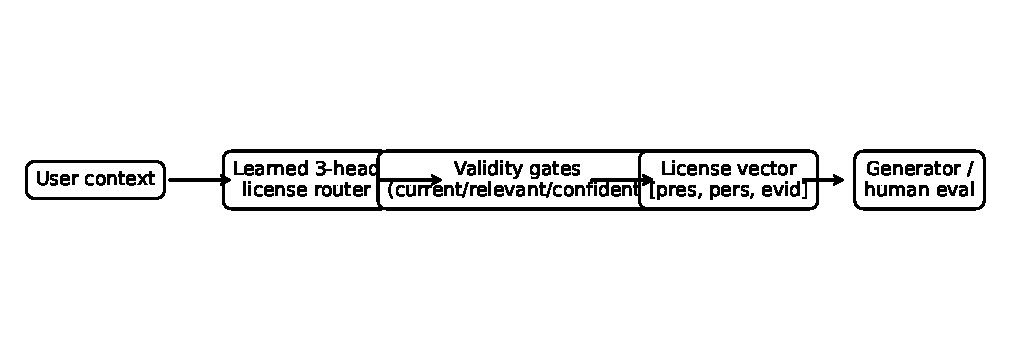
\includegraphics[width=\columnwidth]{figures/architecture.pdf}
\caption{Hybrid PLP learns channel licenses and then applies narrow validity gates. Licensing and downstream generation compliance are evaluated separately.}
\end{figure}

\section{ProvenanceBench}
ProvenanceBench contains 4,800 signal-level examples across travel, calendar, commerce, work, finance, health/wellness, education, and local-life tasks. The benchmark contains four regimes: standard held-out; domain-OOD (finance and education held out from fitting); a compositional test withholding specific provenance/validity conjunctions; and conflicting-evidence groups containing multiple candidate sources for the same personal-state query.

A 552-item blinded human-validation packet is included. Three independent raters per item are recommended, with agreement measured independently for presentation, personalization, and evidence licenses. No human judgments are claimed in the present results.

\subsection{Construction and split discipline}
The 4,800 examples are balanced across eight domains (600 each). The main router uses 1,680 training and 168 validation examples, with 168 ordinary held-out examples, 912 domain-OOD examples, and 720 compositional examples. Conflict selection is separated into 672 training, 192 held-out, and 288 domain-OOD rows because choosing among multiple licensed sources is a distinct decision from determining whether an individual source is licensed at all.

The benchmark includes explicit user statements, inferred signals, third-party messages, tool-verified records, and externally verified records. We intentionally retain both positive and negative evidence cases for the same task/scope families so that a model cannot solve the benchmark by equating relevance with evidentiary permission.

\subsection{Paired provenance intervention}
Standard splits can still encode correlations between source type and task wording. We therefore construct an additional 400 matched pairs (800 examples). Within each pair, task, scope, confidence, currentness, relevance, and surface text are identical; only provenance metadata changes between a licensed and unlicensed source. This intervention is never used for fitting or threshold selection. It is a direct test of causal source sensitivity.

\paragraph{Metrics.} We report exact three-license match, licensed-evidence uptake, unsupported-influence leakage, evidence starvation, conflict-source selection accuracy, and expected calibration error for the evidence head.

\section{Experiments}
Baselines include naive personalization, a fixed firewall, a provenance-only router, and an oracle contract. We compare these to a pure learned PLP router and Hybrid PLP.

\subsection{Training protocol}
Each license head is a class-balanced logistic classifier over TF--IDF signal text, one-hot categorical metadata, and standardized confidence/currentness/relevance features. We choose the binary threshold for each head using validation exact accuracy only; the ordinary test, domain-OOD, compositional, and provenance-intervention sets remain untouched. The hybrid method applies its validity gates after prediction and does not retune thresholds on shifted data. All reported linear-router experiments are rerun over ten solver random states; the metrics are identical across seeds, so the observed shift failures are not initialization noise.

\begin{table*}[t]\centering\small
\begin{tabular}{lccccc}\toprule
Method & ID exact & Domain-OOD exact & Compositional exact & OOD uptake $\uparrow$ & OOD leakage $\downarrow$\\\midrule
Naive personalization & .286 & .368 & .600 & 1.000 & .857\\
Fixed firewall & .571 & .526 & .400 & .000 & .000\\
Provenance-only & .714 & .684 & .600 & .800 & .071\\
Learned PLP & \textbf{1.000} & .842 & .400 & .800 & .143\\
\textbf{Hybrid PLP} & \textbf{1.000} & \textbf{.947} & \textbf{.800} & .800 & \textbf{.000}\\
Oracle & 1.000 & 1.000 & 1.000 & 1.000 & .000\\\bottomrule
\end{tabular}
\caption{Controlled licensing results. Hybrid PLP improves OOD and compositional robustness but does not eliminate evidence starvation; these are routing results, not frontier-model generation results.}
\end{table*}

\subsection{Generalization}
The pure learned router fits the ordinary held-out split but degrades on held-out domains and collapses on the compositional split. Hybrid PLP blocks invalid context more reliably, reaching .947 exact match on domain OOD and .800 on the compositional split, but it cannot recover every licensed-evidence positive missed by the learned router. The result is therefore a robustness improvement, not a solved routing problem.

Against provenance-only on exact license match, the domain-OOD discordant counts are 288 Hybrid-only versus 48 baseline-only (paired exact $p<10^{-14}$); on the compositional split they are 288 versus 144 ($p<10^{-11}$). Item bootstrap intervals are .947 [.933,.962] on domain OOD and .800 [.771,.828] on the compositional split. These quantify benchmark-item uncertainty only.

\subsection{Conflicting evidence}
A separate learned ranker achieves 1.00 selection accuracy on 48 held-out conflict groups and 72 groups from held-out domains. Source authority and freshness are explicit, so this remains a controlled diagnostic rather than a claim about open-ended source reasoning.


\subsection{Feature ablations}
Table~\ref{tab:ablation} shows why a standard split is not enough to establish provenance use. A strict no-provenance ablation removes both source metadata and source-identifying lexical cues; it remains strong on the ordinary benchmark because scope, task, freshness, confidence, and relevance are themselves predictive. The paired provenance intervention is therefore necessary: there, all those variables and surface text are held fixed, and the same ablation falls to chance (0.500 exact match).

\begin{table}[h]\centering\small
\begin{tabular}{lccc}\toprule
Input & ID & OOD & Comp.\\\midrule
Full learned & 1.000 & .842 & .400\\
Hybrid PLP & 1.000 & .947 & .800\\
No provenance cues & .929 & .947 & 1.000\\
Provenance-only & .714 & .684 & .600\\\bottomrule
\end{tabular}
\caption{Exact three-license match on standard splits. The separate paired provenance intervention is required to isolate causal source use.}\label{tab:ablation}
\end{table}

\subsection{Statistical characterization}
We bootstrap benchmark items with 5,000 resamples. Hybrid PLP reaches .947 [ .933, .962 ] exact match on domain OOD and .800 [ .771, .828 ] on the compositional split. Against provenance-only, paired discordant counts are 288/48 on domain OOD ($p<10^{-14}$) and 288/144 on the compositional split ($p<10^{-11}$). The evidence-head expected calibration error rises from .011 on the ordinary held-out split to .157 under domain shift and .486 under compositional shift, showing that confidence degrades before or alongside exact-match failure. These intervals measure benchmark-item uncertainty only; they do not capture model-seed or rater uncertainty.

\begin{figure*}[t]\centering
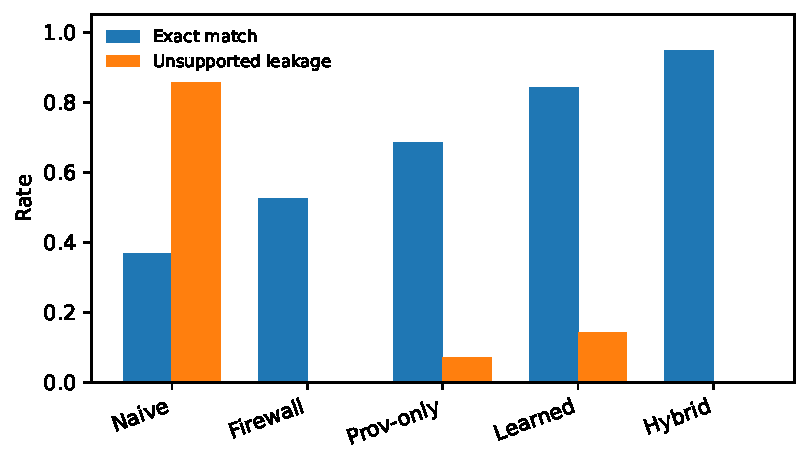
\includegraphics[width=.48\textwidth]{figures/ood_test.pdf}\hfill
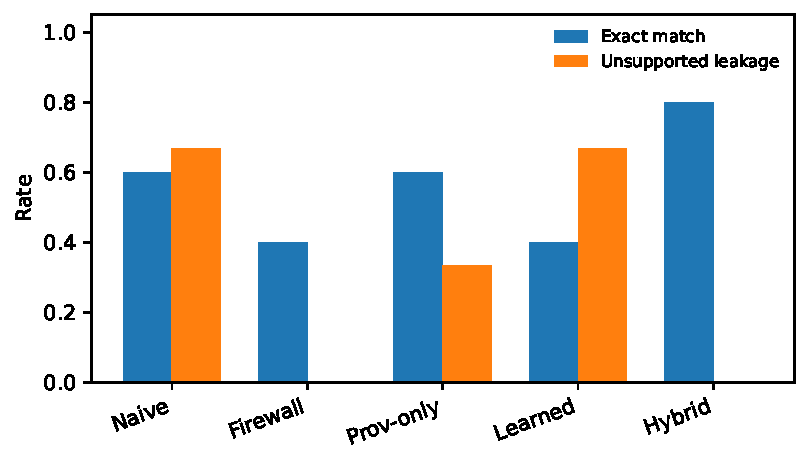
\includegraphics[width=.48\textwidth]{figures/compositional_test.pdf}
\caption{Exact three-license match and unsupported evidence leakage on held-out domains (left) and compositional holdout (right). The pure learned router degrades when validity conditions appear in unseen conjunctions; Hybrid PLP applies explicit validity gates.}
\end{figure*}

\section{Analysis}
\paragraph{Leakage versus starvation.} Naive personalization illustrates leakage; the firewall illustrates starvation. Provenance-only reduces leakage but still mistakes provenance for task validity. Reporting only aggregate accuracy would hide these distinct failure modes.

\paragraph{Why hybridization helps.} The compositional split withholds trusted-but-invalid combinations. Pure supervised learning fails to factor currentness, confidence, and relevance robustly. Explicit validity constraints change the inductive bias: learn ambiguous semantics; encode deliberate invariants.

\paragraph{Paired provenance intervention.} We additionally evaluate 400 matched provenance pairs (800 examples) with identical task, scope, validity metadata, and surface text. Only source provenance changes. A strict no-provenance ablation falls to .500 exact match; learned and Hybrid PLP reach .750, while the narrow provenance-only rule reaches 1.000. The result verifies causal source sensitivity while exposing incomplete transfer to delexicalized contexts.


\subsection{Calibration and error structure}
The evidence head has expected calibration error .011 on the ordinary held-out split, .157 on domain OOD, .486 under compositional shift, and .253 on the paired provenance intervention. The rise in calibration error tracks the shift in exact-match performance and suggests that standard held-out confidence is not a reliable proxy for deployment robustness.

Hybrid PLP's remaining domain-OOD errors are dominated by false negatives for licensed tool-verified world claims: the negative validity gates can prevent unsupported influence but cannot create a positive evidence license that the learned head failed to infer. This motivates a future two-stage design in which evidence acquisition and evidence veto are modeled separately rather than treating gating as a symmetric repair.

\section{Human Validation and Reproducibility}
We prepare a blinded 552-item validation packet sampled across standard, domain-OOD, and compositional conditions. Raters see the task, signal content, scope, provenance metadata, confidence, currentness, and relevance, but not the contract labels or method identity. The planned analysis obtains three independent judgments per item and reports Krippendorff's alpha separately for the three license dimensions. The held-out answer key is stored separately from the rater packet.

The full local experiment is reproducible with a single pipeline. It regenerates the benchmark, fits the learned router, evaluates baselines, runs the conflict ranker, computes bootstrap intervals and paired tests, and builds the human-evaluation packet. Unit tests cover the original behavior suite and learned-router fit. Random seeds are fixed in benchmark generation and statistical resampling.

\paragraph{Oracle decomposition.} The oracle row is not a method claim. It answers a useful systems question: if license inference were perfect, what errors would remain attributable to generation compliance? In future model-level experiments, the same generator should be run with predicted versus oracle licenses so the router and generator can be diagnosed independently.

\section{Threats to Validity}
\textbf{Construct validity.} Contract labels are authored from an explicit policy rather than discovered from users. Human validation is required to determine which cases are genuinely ambiguous. \textbf{External validity.} Natural-language realizations are controlled and do not reproduce the full messiness of production memory stores. \textbf{Metadata availability.} Provenance, confidence, and currentness are explicit in this benchmark but may need to be inferred in deployed systems. \textbf{Policy dependence.} The three hard validity gates reflect a particular design stance; other products may choose different thresholds or escalation rules. \textbf{End-to-end behavior.} A generator can violate a correct license, so licensing scores alone do not establish safe or truthful responses.

\section{Limitations and Next Experiments}
The benchmark is generated from contract archetypes rather than collected from deployed assistants. Human validation is prepared but not yet collected. We do not report end-to-end generation from frontier or open-weight LMs. A submission-level model-behavior study should freeze the benchmark, run real generators, and compare against full-context prompting, retrieval/memory baselines, FPPS-style factuality preservation, cautious context steering, and a Resist-and-Update-inspired control. Feeding oracle licenses to the same generator would separate router error from compliance error.

Real systems also lack perfect provenance metadata. Future work should infer provenance from tool traces and memory stores, quantify provenance uncertainty, and evaluate untrusted content that masquerades as a trusted source. Conflict resolution should also move beyond the simple authority/freshness ordering used here.

\section{Conclusion}
Personalization is not a single scalar controlling how strongly a model mirrors a user. Context can be relevant for style, useful for decisions, and still lack evidentiary standing. PLP turns standing into a learnable interface. The controlled experiments expose a concrete failure of pure supervised licensing under compositional shift and show that a small set of auditable validity constraints can remove measured leakage while still leaving evidence-starvation errors. The current evidence supports a licensing-method and benchmark claim, not an end-to-end frontier-model claim.

\appendix
\section{Artifact Details}
\paragraph{Benchmark record.} Each ProvenanceBench row contains a case identifier, evaluation tier, domain, split, task kind, natural-language signal, semantic scope, provenance class, confidence, currentness, relevance, and three binary license labels. Conflict rows additionally include a conflict-group identifier and a selected-source label. The paired provenance intervention adds a pair identifier so source changes can be audited exactly.

\paragraph{Generation adapter.} End-to-end experiments use a provider-neutral interface \texttt{generate(example, licenses) -> response}. The same frozen case should be run under full-context, predicted-license, and oracle-license conditions. This decomposition distinguishes failures of routing from failures of a generator to obey a correct route.

\paragraph{Human validation.} The blinded packet contains 552 items and excludes contract labels and method identity. Raters independently judge presentation, personalization, and evidence permission. The aggregation script reports nominal inter-rater agreement and majority-vote agreement with the frozen contract labels; no human result is emitted until completed annotations are supplied.

\paragraph{Reproduction.} The repository includes deterministic benchmark generation, learned-router training, threshold selection, OOD and compositional evaluation, the paired provenance intervention, conflict-source evaluation, item-bootstrap intervals, multi-seed stability checks, calibration tables, error exports, and a submission audit. The public claims are generated from these artifacts rather than copied from manually edited tables.

\section*{References}\small
Gihoon Kim et al. \emph{Cautious Context Steering for Language Model Personalization}. arXiv:2608.05813, 2026.\\
Shomik Jain et al. \emph{Interaction Context Often Increases Sycophancy in LLMs}. CHI, 2026.\\
Qiyao Ma et al. \emph{Personalized RewardBench: Evaluating Reward Models with Human Aligned Personalization}. arXiv:2604.07343, 2026.\\
Shuyue Stella Li et al. \emph{HorizonBench: Long-Horizon Personalization with Evolving Preferences}. arXiv:2604.17283, 2026.\\
Zhongxiang Sun et al. \emph{When Personalization Misleads: Understanding and Mitigating Hallucinations in Personalized LLMs}. Findings of ACL, 2026.\\
Sen Yang and Yuen-Hei Yeung. \emph{Resist and Update: Counterfactual Report Coordinates for Incentive-Compatible LLMs}. arXiv:2607.12985, 2026.
\end{document}
